\documentclass[12pt,a4paper]{article}
\usepackage[utf8]{inputenc}
\usepackage{geometry}
\usepackage{graphicx}
\usepackage{xcolor}
\usepackage{titlesec}
\usepackage{fancyhdr}
\usepackage{enumitem}
\usepackage{pgfplots}
\usepackage{fontspec}
\usepackage{setspace}
\usepackage{tabularx}
\usepackage[absolute,overlay]{textpos}
\pgfplotsset{compat=1.18}

% Define custom colors
\definecolor{hydrosensblue}{RGB}{37, 51, 114}
\definecolor{hydrosenscyan}{RGB}{81, 186, 215}

% Page margins
\geometry{
    top=2cm,
    bottom=2cm,
    left=2cm,
    right=2cm
}

% Load custom fonts
\newfontfamily\titlefont[
  Path = fonts/,
  UprightFont = JosefinSlab-Regular,
  BoldFont = JosefinSlab-Bold
]{Josefin Slab}

\newfontfamily\subtitlefont[
  Path = fonts/,
  UprightFont = LibreBaskerville-Regular,
  BoldFont = LibreBaskerville-Bold
]{Libre Baskerville}

\newfontfamily\contentfont[
  Path = fonts/,
  UprightFont = LibreBaskerville-Regular
]{Libre Baskerville}

% Custom styling commands
\newcommand{\HydroTitle}[1]{%
    {\titlefont\color{hydrosensblue}\bfseries\fontsize{60pt}{40pt}\selectfont #1}
}

\newcommand{\HydroSubtitle}[1]{%
    {\subtitlefont\color{hydrosensblue}\bfseries\fontsize{16pt}{20pt}\selectfont #1}
}

\newcommand{\HydroContent}[1]{%
{\contentfont\color{black}\normalfont\fontsize{16pt}{20pt}\selectfont #1}
}

% Fancy header/footer
\pagestyle{fancy}
\fancyhead{}
\fancyfoot{}
\renewcommand{\headrulewidth}{0pt}
\renewcommand{\footrulewidth}{0pt}

% Section title formatting
\titleformat{\section}
  {\normalfont\Large\bfseries\color{hydrosensblue}\titlefont}
  {}
  {0em}
  {}[\titlerule]

\titleformat{\subsection}
  {\normalfont\large\bfseries\color{hydrosenscyan}\subtitlefont}
  {}
  {0em}
  {}

% Document begin
\begin{document}
% Intro start
\begin{titlepage}
\begin{center}
\begin{minipage}{0.75\textwidth}
    \raggedright
    \HydroTitle{RSS\vspace{0.5cm}}\\[0.1cm]
    \HydroTitle{HYDROSENS}
\end{minipage}
\hfill
\begin{minipage}{0.15\textwidth}
    
\includegraphics[width=\linewidth]{images/logo.png}
\end{minipage}
\end{center}

% Seperator line
\vspace{0.5\baselineskip}
\noindent\color{hydrosenscyan}\rule{0.25\textwidth}{3pt}
\vspace{1\baselineskip}

% Subtitle
\noindent
\HydroSubtitle{ENVIRONMENTAL MONITORING REPORT}

\vspace{1cm}

% Region and Time Period
\noindent
\HydroSubtitle{REGION:}
\HydroContent{District 7 - Ho Chi Minh}

\vspace{0.2cm}

\noindent
\HydroSubtitle{\textbf{TIME PERIOD:}}
\HydroContent{10 Apr - 35 May 2025}

\vfill

% Decorative Image with circle crop at bottom right
\begin{tikzpicture}[remember picture, overlay]
    % === Background block (hydrosenscyan), half the height of the circle ===
    \fill[hydrosenscyan]
        ([xshift=-\paperwidth,yshift=10cm]current page.south east) rectangle
        ([xshift=0cm,yshift=0cm]current page.south east); % 2cm height = half of 4cm radius circle

    % === Circular clipped image ===
    \begin{scope}
        \clip (current page.south east) ++(-4cm, 4cm) circle (20cm); % Adjust position and size
        \node at ([xshift=-7cm, yshift=7cm]current page.south east)
            {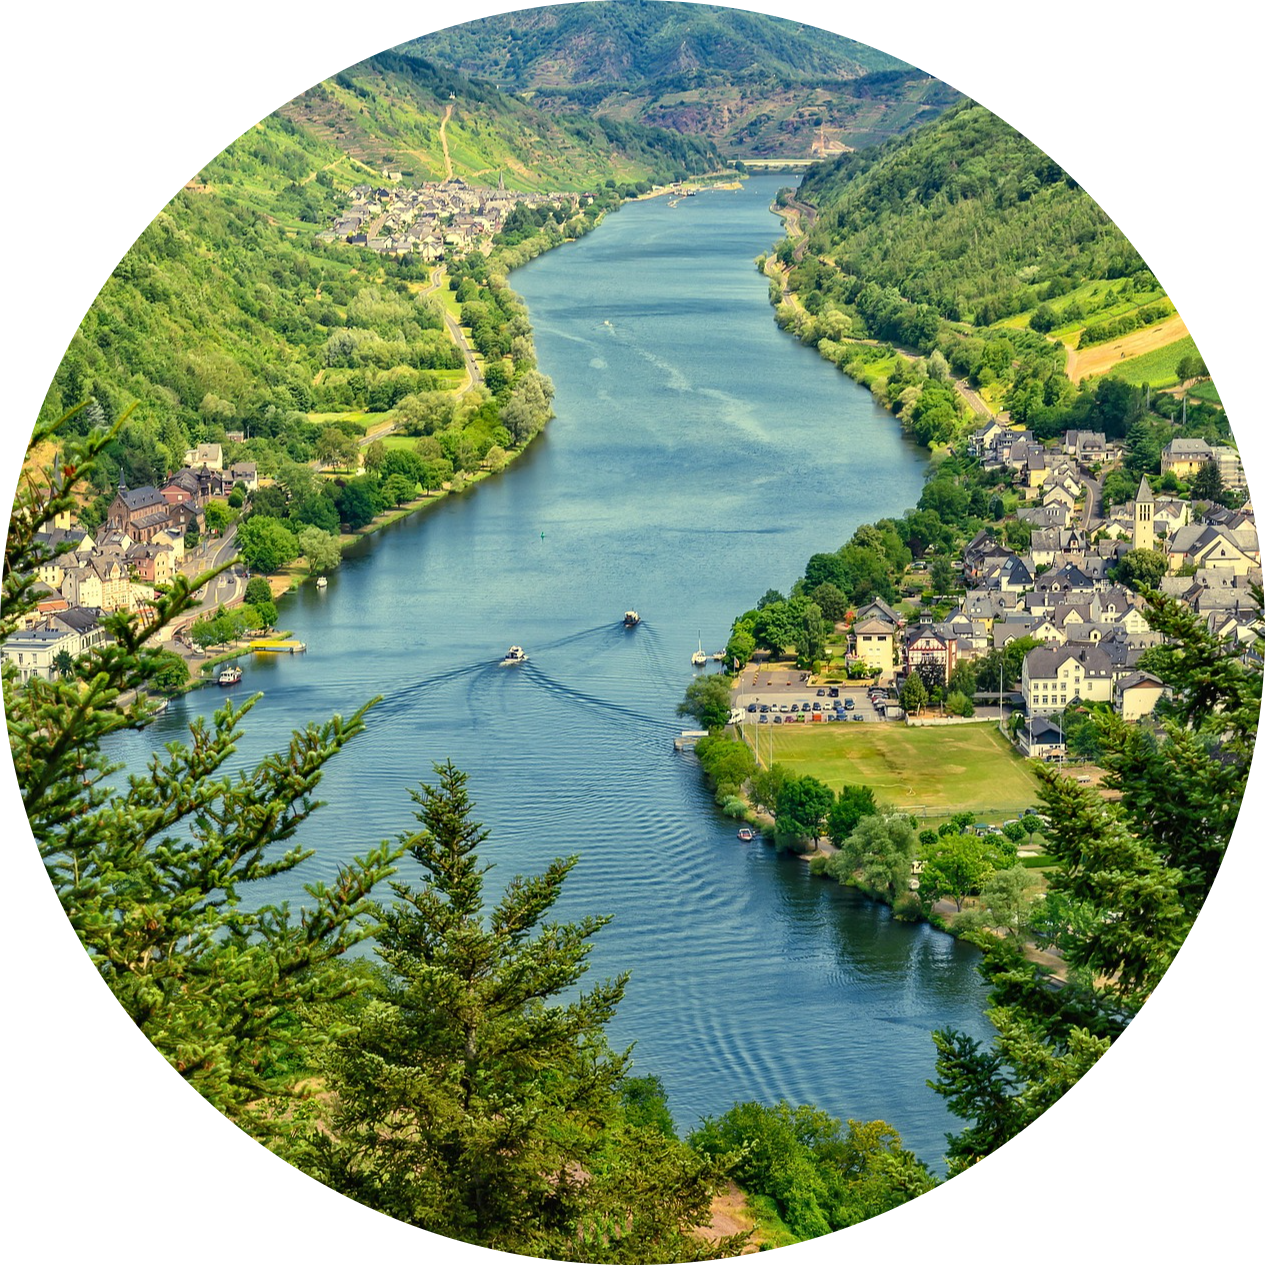
\includegraphics[width=20cm]{images/intro.png}}; % Adjust image width
    \end{scope}
\end{tikzpicture}
\end{titlepage}


% --- Overview Page ---

% Overview Title
\noindent
\HydroTitle{OVERVIEW}

\vspace{0.3cm}

% Light blue line under the heading
\vspace{0.5\baselineskip}
\noindent\color{hydrosenscyan}\rule{0.25\textwidth}{3pt}
\vspace{1\baselineskip}

% Body text
\noindent   
\begingroup
  \setstretch{1.5}%
  \contentfont
  \color{black}%
  \normalfont
  \fontsize{16pt}{20pt}\selectfont
This report provides a comprehensive assessment of six key environmental metrics—NDVI, Vegetation Fraction, Soil Moisture, Precipitation, Temperature, and Curve Number—for a selected geographic area over the course of 2024. The objective is to deliver intuitive insights into the region’s vegetation health, water balance, and climate dynamics, enabling both technical and non-technical stakeholders to make informed decisions.
\par
\endgroup

\begin{tikzpicture}[remember picture, overlay]
    \node[anchor=south, yshift=1.5cm] at (current page.south) {
        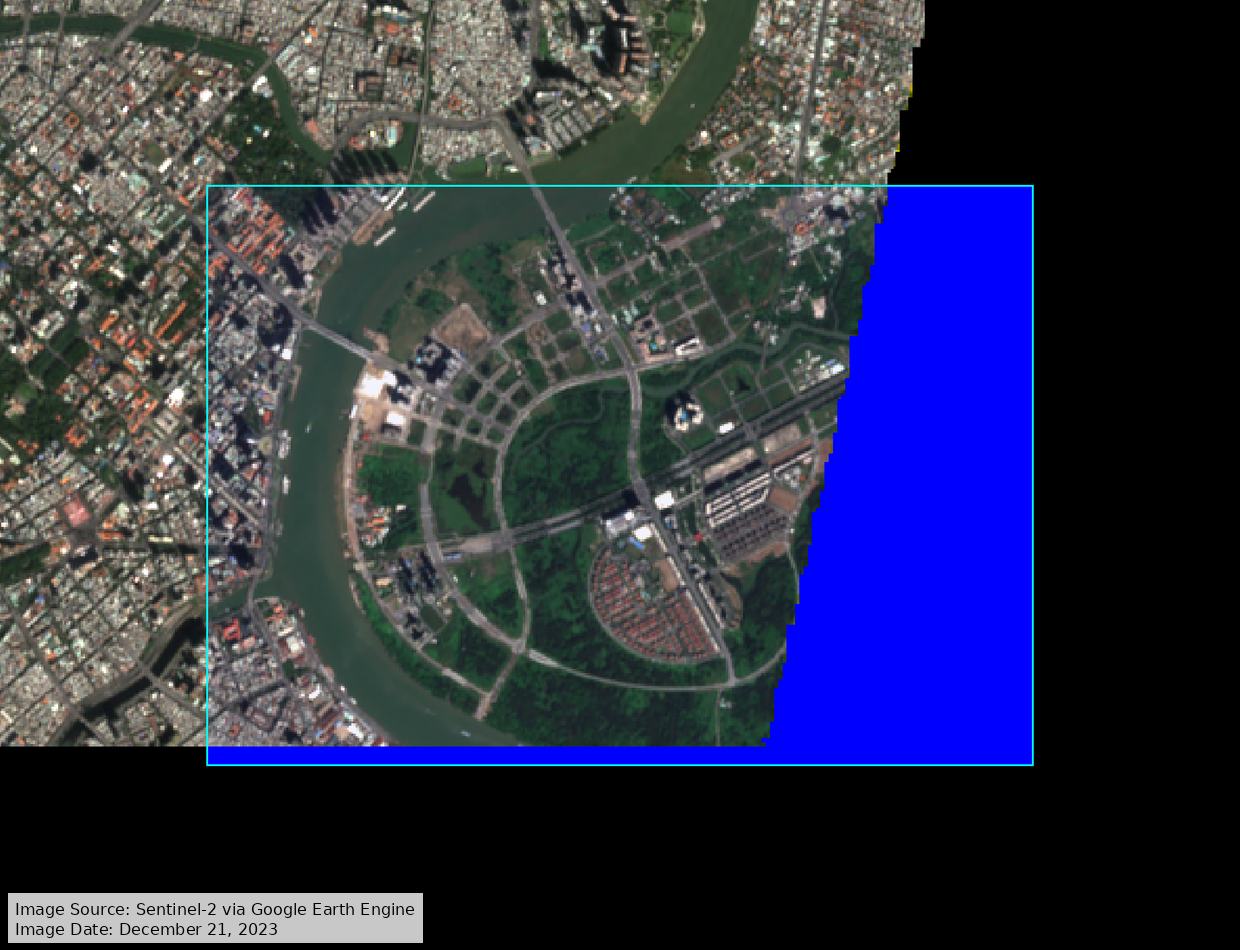
\includegraphics[width=\textwidth, height=50cm, keepaspectratio]{images/region_screenshot.png}
    };
\end{tikzpicture}

% Key insights start
\clearpage
\noindent
\begin{minipage}[t]{0.6\textwidth}

\HydroTitle{KEY\vspace{0.5cm}}\\ % Adds vertical space *inside* the title box
\HydroTitle{INSIGHTS}

  \vspace{0.5\baselineskip}
  \color{hydrosenscyan}\rule{0.25\textwidth}{3pt}
  \vspace{1\baselineskip}

  \setstretch{1.5}
  \HydroContent{\textbf{1. Healthy but Moderate Vegetation}\\
  Vegetation indicators (NDVI and Vegetation Fraction) remained consistently moderate, peaking during spring and early summer.}

  \vspace{0.6cm}

  \HydroContent{\textbf{2. Adequate Soil Moisture}\\
  Soil moisture levels were stable and adequate throughout the year, supporting consistent plant growth.}

  \vspace{0.6cm}

  \HydroContent{\textbf{3. Seasonal Rainfall Distribution}\\
  Precipitation followed a clear seasonal pattern, with wetter periods in early autumn and late summer, and noticeably drier months during mid-year.}

  \vspace{0.6cm}

  \HydroContent{\textbf{4. Temperate Climate Patterns}\\
  Average temperature hovered around 22°C with warm peaks early in the year and cooling mid-year, consistent with subtropical seasonal cycles.}

  \vspace{0.6cm}

  \HydroContent{\textbf{5. Moderate Runoff Risk}\\
  Curve Number values indicate the area has mixed surface permeability—neither highly absorbent nor heavily sealed—suggesting }
\end{minipage}%
\hfill
\begin{minipage}[t]{0.25\textwidth}
% Background image on right half
\begin{tikzpicture}[remember picture,overlay]
  \node[anchor=north east, inner sep=0pt] at (current page.north east)
    {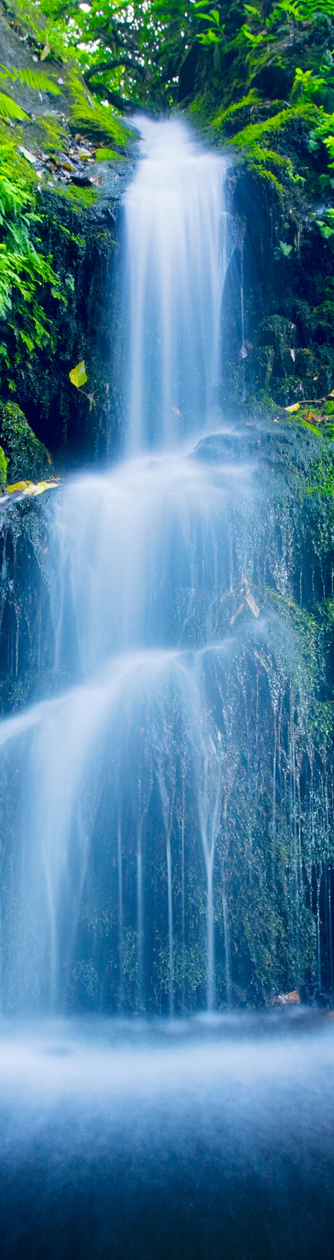
\includegraphics[height=\paperheight]{images/waterfall.png}};
\end{tikzpicture}

\end{minipage}

\clearpage
% Metric start (1 example)
\clearpage
% Top border line
\vspace*{-0.5cm}
\noindent
\color{teal}\rule{\textwidth}{2pt}
\vspace{0.3cm}

% Header
\noindent
\begin{tabular*}{\textwidth}{@{\extracolsep{\fill}} l r }
\textsf{\textbf{\small STATISTICS}} & \textsf{\textbf{\small PAGE 05}} \\
\end{tabular*}

\vspace{0.7cm}

% Title and Mean Value aligned on the same line
\noindent
\begin{tabularx}{\textwidth}{@{}X r@{}}
  \begin{minipage}[t]{0.65\textwidth}

\begingroup
  \setstretch{1.5}%
  \titlefont
  \color{hydrosensblue}%
  \fontsize{40pt}{30pt}
  \bfseries\selectfont
  \noindent   
NORMALIZED DIFFERENCE VEGETATION INDEX
\par
\endgroup

    \vspace{0.3cm}
    \par \textit{Indicates vegetation health from 0 to 1.}
  \end{minipage}
  &
  \begin{minipage}[t]{0.35\textwidth}
  {\subtitlefont\color{hydrosenscyan}\bfseries\fontsize{50pt}{40pt}\selectfont 0.36}\\[0.3cm]
    \HydroSubtitle{\textbf{MEAN VALUE}}\\[-0.3cm]

\svnoindent\color{hydrosenscyan}\rule{5.2cm}{2pt}\\[0.3cm]
    \setstretch{1.5}
    \HydroContent{An average NDVI of 0.36 suggests moderate vegetation density, indicating some vegetative activity but potentially below optimal levels.}
  \end{minipage}
\end{tabularx}

\vspace{2cm}

% Time series insight and chart image on same line
\noindent
\begin{tabularx}{\textwidth}{@{}X r@{}}
  % Left column – Time Series Insight block, aligned top
  \begin{minipage}[t]{0.48\textwidth}
    \vspace{0pt} % ensure top alignment
    \HydroSubtitle{TIME SERIES INSIGHT}\\[-0.5ex]
    \noindent\color{hydrosenscyan}\rule{6cm}{2pt}
    \vspace{0.3cm}

    \setstretch{1.5}
    \HydroContent{NDVI values fluctuated between 0.29 and 0.43 during the reporting period. An increase in early January suggests a positive response to environmental factors or management practices, followed by a gradual decline towards the end of January.}
  \end{minipage}
  &
  % Right column – image aligned top
  \begin{minipage}[t]{0.48\textwidth}
    \vspace{0pt}
    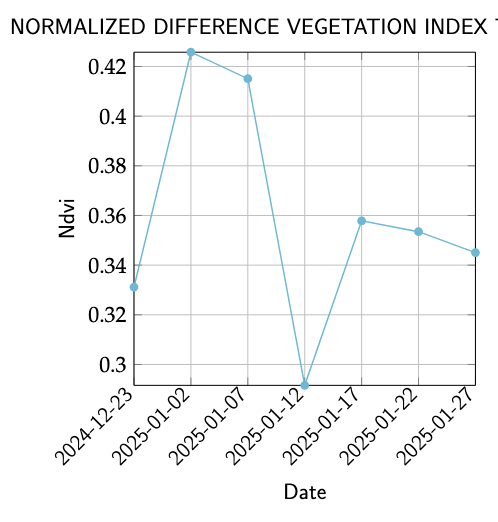
\includegraphics[width=\linewidth]{images/metric.png}
  \end{minipage}
\end{tabularx}

\vfill

% Bottom border line
\noindent\color{teal}\rule{\textwidth}{2pt}
% Action start
\newpage

% Action Plans Page
\vspace*{-0.5cm}
\noindent\HydroTitle{ACTION PLANS}

% Light blue line under the heading
\vspace{0.5\baselineskip}
\noindent\color{hydrosenscyan}\rule{0.25\textwidth}{3pt}
\vspace{2\baselineskip}

\noindent\begin{minipage}{\textwidth} % \noindent ensures the minipage starts flush with the left margin
\setstretch{1.5}
\color{black}
\begin{itemize}[leftmargin=*, rightmargin=0pt] % Adjusts list margins
    \item \HydroContent{Implement efficient irrigation practices to address the lack of rainfall and ensure adequate water supply for vegetation.}
    \item \HydroContent{Monitor soil moisture levels regularly and adjust irrigation strategies as needed.}
    \item \HydroContent{Consider implementing soil conservation measures to minimize runoff potential and improve water infiltration.}
    \item \HydroContent{Select drought-resistant vegetation species for future plantings to reduce water demand.}
    \item \HydroContent{Conduct further investigation into the factors causing NDVI fluctuation and the runoff potential change.}
\end{itemize}
\end{minipage}

% --- Image at the bottom of the page (no margins) ---
\begin{tikzpicture}[remember picture,overlay]
    \node[anchor=south west, inner sep=0pt, outer sep=0pt] at (current page.south west) {
        
\includegraphics[width=\paperwidth,height=10cm]{images/action.jpg} % Adjust height as needed
    };
\end{tikzpicture}
% --- End of image block ---
\end{document}